\input{preambulo.tex}

% Titulo
\title[DHCP] {DHCP del Internet Software Consortium}
\author[Carlos Maldonado]{ info@covetel.com.ve \inst{1}}
\subtitle{Fundamentos y Configuraciones Típicas}
\institute[covetel.com.ve]{ \inst{1} Cooperativa Venezolana de Tecnologías Libres R.S. }
\date

\begin{document}

\begin{frame} % (fold)
    \titlepage 
\end{frame}

\begin{frame} % (fold)
    \tableofcontents
\end{frame}

\section{Linux en nuestro entorno de pruebas} % (fold)

\subsection{Usando el entorno de pruebas} % (fold)

\begin{frame}[allowframebreaks,fragile]{Accediendo al entorno de pruebas}

    En nuestro caso trabajaremos con máquinas virtuales hospedadas en el
    servidor con el IP proveído por el instructor. Dos máquinas virtuales para
    cada participante, una que actuará como servidor y otra como
    cliente. Cada par de máquinas esta conectada entre sí por un
    \textit{bridge virtual} que les permite intercambiar paquetes entre ellas
    sin contaminar con \textit{broadcast} al resto de las máquinas virtuales de
    los demás participantes\\[0.2cm] 

    Para conectarse al servidor donde están hospedadas las máquinas virtuales,
    es preciso usar el comando:\\[0.2cm]

\begin{verbatim}
    ssh root@161.196.33.115
\end{verbatim} 

    \framebreak

    Dependiendo de la ubicación de los participantes en el
    laboratorio, se hará la asignación de máquinas en pares,
    todas pueden ser visualizadas con el comando:\\[0.2cm]

\begin{verbatim}
    vzlist
\end{verbatim} 
     
    Las máquinas listadas se encuentran diferenciadas por el identificador
    'CTID' en los campos del tope de la lista.  Cada participante tiene
    asignadas dos máquinas, una en la serie 31x y una en la serie 32x.
    Las máquinas de la serie 31x están destinadas a ser máquina servidor
    y las máquinas de la serie 32x están diseñadas como máquina cliente.\\[0.2cm]

    El comando usado para acceder a las máquinas virtuales, es el siguiente:

\begin{verbatim}
    vzctl enter [CTID]
\end{verbatim}

    Esto le ubicará dentro de la máquina virtual indicada por 'CTID'.
    Si desea saber en que host esta la sesión actual, puede usar el
    comando:\\[0.2cm]

\begin{verbatim}
    uname -a
\end{verbatim}

    Cada una describe si es máquina cliente o servidor en su hostname.
    
\end{frame}

\subsection{Comandos básicos} % (fold)

\begin{frame}[allowframebreaks,fragile]{Comandos básicos requeridos} 

    Los ejercicios de este curso requerirán el uso básico de los siguientes
    comandos:

    \begin{verbatim}
    man : despliega la hoja de manual de un comando
    cd : cambia el directorio actual
    nano / vim : editores de texto en línea de comando
    ls : lista archivos y directorios
    sort :  ordena alfabética o numéricamente un conjunto de líneas
    cut : selecciona campos de un archivo o salida
    uniq : elimina las lineas repetidas adyacentes
    grep : busca/filtra una cadena en un archivo o salida
    tail : muestra la parte final de un archivo o salida
    head : muestra la parte superior de un archivo o salida
    wc : cuenta la cantidad de líneas, palabras o caracteres
    \end{verbatim}

    \framebreak

    Tome en cuenta que la salida de un comando, puede ser la entrada de otro,
    comunicándolos con un caracter 'pipe' entre ellos, por ejemplo:

    \begin{verbatim}
    grep DHCP dhcpd.log | wc -l
    \end{verbatim}

    Se encarga de contar todas las coincidencias de la cadena DHCP en el
    archivo dhcp.log

    Usando el comando 'man' se puede leer el manual de cada uno de los otros
    comandos y así tener una referencia sobre que switches y opciones están
    disponibles en cada uno, cada manual es autocontenido. Para leer el manual
    del comando wc, se necesitaría tipear:

    \begin{verbatim}
    man wc
    \end{verbatim} 

\end{frame}

\begin{frame}

    Pongámonos a prueba con las siguientes prácticas, para aprender o recordar
    lo que necesitaremos en lo sucesivo. Si usted es capaz de resolver estos
    ejercicios en una sola línea, sin leer páginas de manual, puede
    saltarse esta sección de introducción. \\[0.2cm]

    \begin{itemize}
        \item Contar la cantidad de directorios que tiene la raíz del sistema
        de archivos
        \item Contar la cantidad de líneas que contienen la palabra 'kernel' en
        /var/log/syslog
        \item Extraer las direcciones IP configuradas en la máquina local (sin
        espacios o caracteres adicionales) (tip: comando /sbin/ifconfig)
        \item Extraer las líneas que contienen la palabra error (sin prestar
        atención a mayúsculas o minúsculas) del comando dmesg
        \item Contar la cantidad de líneas con DHCPDISCOVER que tiene el
        archivo dhcp.log para el día 20 de Diciembre
        \item Emitir una lista de todos los mensajes de tipo DHCP registrados
        en el archivo dhcp.log y que cantidad de cada uno existen allí
    \end{itemize}
    
\end{frame}

\subsection{Instalación de aplicaciones} % (fold)

\begin{frame}[allowframebreaks,fragile]{Instalación de paquetes}

    La mayoría de las distribuciones Linux, posee un sistema de paquetes para
    la instalación de aplicaciones y sus datos. En el caso de Debian, el
    manejo de paquetes se realiza con apt y sus herramientas relacionadas.\\[0.2cm]

    En nuestro caso usaremos de manera limitada el sistema de paquetes, ya que
    nuestras máquinas virtuales no están conectadas la Internet, ni tienen
    disponible un repositorio de paquetes. Solo instalaremos el paquete con el
    comando:\\[0.2cm]

\begin{verbatim} 
    dpkg -i [nombre del archivo del paquete]
\end{verbatim}

    Con acceso normal a un repositorio, dicha operación debería realizarse con los
    comandos:\\[0.2cm]

\begin{verbatim} 
    apt-get update # para actualizar la base de datos de paquetes
    apt-get install isc-dhcp-server # instala el servidor DHCP del ISC
\end{verbatim}


\end{frame}


\section{Introducción a DHCP}

\subsection{Fundamentos de DHCP} % (fold)

\label{sub:Fundamentos de DHCP}

% subsection Fundamentos de DHCP (end)

\begin{frame}[allowframebreaks,fragile]{Dynamic Host Control Protocol} % (fold)
    Dynamic Host Control Protocol o \textbf{DHCP} (en castellano, protocolo de
    control de máquinas dinámicas) es el protocolo usado para asignar
    direcciones de manera automática y dinámica en redes de computadores. \\[0.2cm]

    Desarrollado por el Dynamic Host Configuration Working Group del IETF desde
    1993 a 1997 y reflejado en los \textbf{RFC 1351} y \textbf{RFC 2616}. \\[0.2cm]

    El protocolo DHCP esta diseñado para satisfacer la demanda de operaciones
    donde es necesario automatizar la configuración de computadores en red. \\[0.2cm]

    La máquina que efectúa la petición se le conoce como \textit{Cliente} y
    existen implementaciones de el programa cliente en prácticamente cualquier
    plataforma de hardware y sistema operativo. \\[0.2cm]

    La información transmitida entre cliente y servidor son paquetes no
    superiores a la MTU \textbf{Maximum Transfer Unit} del protocolo de capa 2
    que use la red, tipicamente este protocolo es Ethernet o una de
    sus variantes más rápidas. \\[0.2cm]

    La razón para esta limitación estriba en que es necesario que toda la
    información pueda ser enviada en un solo paquete que será enviado en
    modo broadcast, dado que la máquina cliente que hace la petición, no tiene
    una dirección de red (capa 3) con la cual enviar su paquete y recibir una
    respuesta usando dicha dirección. \\[0.2cm]

    DHCP es un protocolo \textbf{sin estado} (\textit{Stateless}), esto quiere
    decir que no guarda ninguna información sobre conexiones anteriores. La
    única información que se almacena, son las direcciones que se han entregado
    (arrendado) a los distintos clientes que han hecho peticiones.\\[0.2cm]

    Además de la dirección IP, existen otros valores de configuración que se
    pueden establecer mediante el uso de DHCP. Routers por omisión, DNS
    primario y secundario, máscara de red, dirección de broadcast y servidores
    WINS, entre otras.\\[0.2cm]

\end{frame} 

\begin{frame}[allowframebreaks,fragile]{Mitos comunes detrás del DHCP} % (fold)

    \textbf{Exceso de tráfico broadcast:} es un mal concepto ampliamente
    difundido, que DHCP generaría una gran cantidad de tráfico \textit{broadcast},
    en realidad la cantidad de \textit{broadcast} es mínima. En el peor de los
    casos, con un cliente de capacidades limitadas, el intercambio de paquetes
    broadcast serían cuatro.\\[0.2cm]
    
    En el mejor de los casos, que comprende una gran mayoría de los sistemas
    operativos, el cliente necesitaría solo enviar un paquete \textit{broadcast}
    y no requeriría una respuesta \textit{broadcast}. La mayoría de los servidores
    también pueden responder en modo \textit{unicast}.\\[0.2cm]

    Otro mito es que el \textit{broadcast} abarcaría toda red corporativa,
    cuando en realidad, solo esta limitado al segmento de red donde la máquina
    cliente del DHCP está conectada. El resto del tráfico sería \textit{unicast}.\\[2cm]

    \textbf{Exceso de carga en el servidor:} otro concepto común es que un
    servidor DHCP necesitaría mucho poder de cómputo para brindarle servicio a
    miles de máquinas. Sin embargo, es posible darle servicio a alrededor de
    10.000 clientes con una máquina 486 con Linux.\\[0.2cm]

\end{frame} 

\subsection{Asignación de direcciones} % (fold)

\begin{frame}[allowframebreaks,fragile]{Tipos de asignación} % (fold)
    \textbf{Asignación estática:} el servidor recibe una listado con
    información que identifica a los clientes DHCP. Dicho listado permite
    diferenciar a cada uno de los clientes. Para cada identificador, se
    establece una dirección IP que debe ser asignada a dicho cliente.
    Si el cliente es móvil, debe haber una dirección para dicho
    dispositivo en cada rango de la red. \\[0.2cm]

    \textbf{Asignación dinámica:} el servidor recibe un rango de direcciones
    para cada segmento de red donde se espera que hayan clientes DHCP. Cuando
    el cliente solicita una dirección, el servidor consigue una dirección
    disponible en dicho segmento de red para entregarla al cliente.\\[0.2cm]

    \textbf{Asignación automática:} el servidor asigna una dirección de la
    misma manera que en el método dinámico, solo que dicha dirección se asigna
    de manera permanente al mismo cliente. Una manera aproximada de usar dicho
    modo de asignación es utilizar \textit{leases} muy largos.\\[0.2cm]

    \framebreak

    \textbf{Asignación híbrida:} existen una variedad de métodos híbridos que
    son posibles con DHCP. Por ejemplo una estrategia común es asignar
    direcciones fijas a los clientes DHCP registrados, permitiendo que los
    cliente DHCP no registrados adquieran direcciones IP asignadas de manera
    dinámica.\\[0.2cm]

    Cual de estas estrategias ha de utilizarse en una red en particular, es una
    decisión que queda de parte del administrador. Obviamente, mantener un
    registro de todos los clientes DHCP conectados en una red es una carga de
    trabajo considerable que en algunos entornos vale la pena.\\[0.2cm]

    Es necesario resaltar que DHCP no debe usarse como mecanismo de seguridad,
    si el cliente DHCP elige no seguir el protocolo, el administrador puede
    hacer poco más que, detectar el dispositivo y bloquearlo. Usar control de acceso
    puede ser conveniente, pero no evita el acceso no autorizado a una
    red.\\[0.2cm]
    
\end{frame}

\subsection{Funciones principales del DHCP} % (fold)
\label{sub:Funciones principales del DHCP}

% subsection Funciones principales del DHCP (end)

\begin{frame}{Arrendado (leasing)} % (fold)

    Tal y como se explicó que el servidor DHCP es \textit{Stateless} y
    opera de manera automática, este no puede saber que ha pasado con los
    dispositivos después de que se les asigna una dirección. En vez de asignar una
    dirección IP a cada cliente hasta que este termine de usarla, el servidor
    DHCP asigna una dirección con un \textit{lease} y el cliente esta
    autorizado a usarla hasta el final de la duración de dicho
    \textit{lease}.\\[0.2cm]


\end{frame}

\begin{frame}{Reclamación (reclamation)} % (fold)

    Al restringir los clientes a usar direcciones IP, solo hasta que expiren
    los \textit{leases} y al proveer un mecanismo para que actualicen los
    \textit{leases} mientras estén activos y conectados a la red, DHCP permite
    'reclamar' las direcciones IP que no están en uso. Si un dispositivo esta
    apagado por un periodo extendido de tiempo, debe contactar al servidor DHCP
    y solicitar una dirección cuando se activa. Si la dirección anterior no
    está disponible, se le ofrece una nueva dirección. Esto evita la mayoría de
    los conflictos de asignación de direcciones.

\end{frame}

\begin{frame}{Liberación (release)} % (fold)

    Un cliente puede renunciar a su \textit{lease} sobre una dirección, antes
    de que expire, por ejemplo cuando una máquina va a moverse de una red a
    otra, de manera que el servidor sepa que la dirección queda disponible
    inmediatamente para ser reasignada. Algunos clientes DHCP pueden
    configurarse para renunciar a su dirección cada vez que la máquina se
    apaga. El cliente no espera una respuesta a dicha transacción.

\end{frame}

\begin{frame}{Descripción de servicios} % (fold)

   Además de distribuir direcciones IP, DHCP permite configurar información que
   sea distribuida en la forma de opciones de DHCP, incluyendo las siguientes:

   \begin{itemize}
       \item Dirección del router por omisión
       \item Dirección(es) de servidor(es) DNS
       \item FQDN al que debe pertenecer la máquina
       \item Nombre del servidor NTP para sincronizar la hora
       \item Nombre del servidor para descargarse una imagen boot por TFTP
       \item Nombre del archivo para hacer boot de una máquina (para dispositivos que inician
       cargando archivos desde un dispositivo de almacenamiento disponible en
       la red)
       \item Nombre del sistema de archivos y servidor de swap (para clientes
       DHCP sin disco)
   \end{itemize}

\end{frame}

\subsection{Ejemplo inicial de funcionamiento} % (fold)
\label{sub:Ejemplo inicial de funcionamiento}

% subsection Ejemplo inicial de funcionamiento (end)

\begin{frame}[allowframebreaks,fragile]{Ejemplo básico de direccionamiento DHCP} % (fold)

    A continuación veremos una red de ejemplo en la organización ficticia MAY,
    cinco segmentos de red, todos ellos conectados entre si por un router que
    a su vez los conecta a Internet. Cuatro segmentos de red son usados por las
    estaciones de escritorio del personal de la empresa, el segmento restante
    se usa para los servidores que se encuentran alojados en el centro de
    datos. 

    \begin{figure}
    \begin{center}

    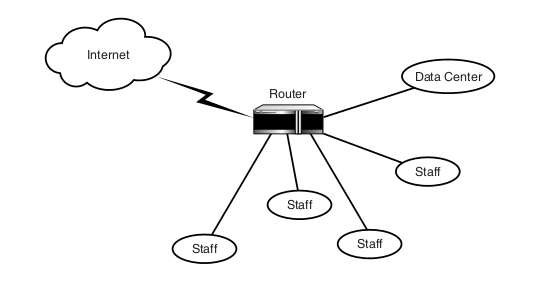
\includegraphics[scale=0.65]{images/2-1.png}
    \caption{Diagrama de la red MAY}
    \label{MAY-1}

    \end{center}
    \end{figure}

    El administrador de la red, ha obtenido cinco redes IP clase C desde la
    192.168.11.0 hasta la 192.168.15.0 y se han asignado a los segmentos de red
    como se muestran en la siguiente figura 

    \begin{figure}
    \begin{center}

    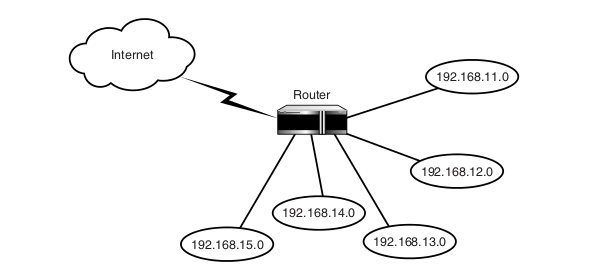
\includegraphics[scale=0.65]{images/2-2.png}
    \caption{Diagrama de la red MAY con direcciones de red}
    \label{MAY-2}

    \end{center}
    \end{figure}

    El objetivo es lograr que un servidor DHCP se encargue de gestionar la
    configuración de las computadoras conectadas a la red MAY. Ahora
    describiremos brevemente las interacciones entre un computador de
    escritorio y el servidor DHCP de la red MAY, en las siguientes instancias:

    \begin{itemize}
        \item Cuando un computador se conecta por primera vez a la red MAY
        \item Cuando un computador se reinicia
        \item Cuando un computador es cambiado de ubicación dentro de la red MAY
        \item Cuando un computador es eliminado de la red MAY
    \end{itemize}

    \begin{figure}
    \begin{center}

    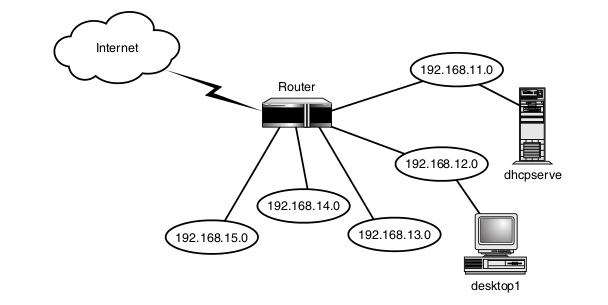
\includegraphics[scale=0.65]{images/2-3.png}
    \caption{Diagrama de la red MAY - Cliente - Servidor }
    \label{MAY-3}

    \end{center}
    \end{figure}

\end{frame}

\begin{frame}[allowframebreaks,fragile]{Cuando un computador se conecta por primera vez a la red
MAY} % (fold)

    Cuando \textit{desktop1} se conecta por primera vez a la red MAY, necesita
    contactar al servidor DHCP para obtener una dirección IP y otros parámetros
    de configuración. Para ubicar un servidor DHCP, \textit{desktop1} envía un
    mensaje broadcast \textit{desktop1} para ubicar potenciales servidores
    DHCP en la red MAY.\\[0.2cm]

    Luego \textit{dhcpserve} recibe este \textit{broadcast} y responde a
    \textit{desktop1} identificándose como un servidor DHCP. Como
    \textit{desktop1} y \textit{dhcpserve} están en distintos segmentos de red,
    el router actuando como \textit{relay agent}, reenvia los mensajes entre
    ambos computadores. En diapositivas posteriores, se explicará esto con
    detalle.\\[0.2cm]

    Después de \textit{dhcpserve} recibir el mensaje inicial de
    \textit{desktop1}, \textit{dhcpserve} selecciona una dirección IP
    (192.168.12.25) que es adecuada para la red 192.168.12.0 a la que \textit{desktop1} está
    conectada. Otros parámetros de configuración son enviados adicionalmente, como por
    ejemplo: la máscara de red, la dirección de la interfaz de red del router
    en la red 192.168.12.0 y la dirección del servidor DNS en la red
    MAY.\\[0.2cm]

    \textit{dhcpserve} usa las reglas de configuración del cliente, definidas
    por el administrador de la red y la información enviada por el
    \textit{relay agent} para determinar dichos parámetros. Luego responde con
    un mensaje de 'oferta' que contiene la dirección seleccionada y los
    parámetros a \textit{desktop1}.\\[0.2cm]

    Despues de \textit{desktop1} recibir el mensaje de 'oferta' de
    \textit{dhcpserve}, envía un mensaje en forma de \textit{broadcast}
    solicitando la dirección IP que le ha sido ofrecida. Así el servidor
    \textit{dhcpserve} confirma que la dirección está aún disponible y envía
    los parámetros a \textit{desktop1}.\\[0.2cm]

    Cuando el mensaje llega, el software cliente DHCP extrae los parámetros de
    configuración y configura el stack IP del computador con la información
    recibida, tan pronto el IP stack está configurado, se puede usar la red
    normalmente. Igualmente el software guarda dichos valores de configuración
    para su uso posterior, en un archivo en \textit{desktop1}.\\[0,2cm]

\end{frame}


\begin{frame}[allowframebreaks,fragile]{Cuando un computador se reinicia} 

    Cuando \textit{desktop1} es reiniciado o encendido al inicio de la jornada,
    se leen los valores de configuración que fueron recibidos y guardados la
    última vez y se intenta contactar a \textit{dhcpserve} para confirmar si
    dicha configuración puede ser usada aún.\\[0,2cm]
    
    En caso de que \textit{desktop1} no reciba una respuesta de
    \textit{dhcpserve} y el \textit{lease} de su dirección previa no haya
    expirado, asume que se encuentra aún en el mismo segmento de red y sigue
    usando la IP 192.168.12.25, con el resto de valores asignados previamente
    por \textit{dhcpserve}.\\[0.2cm]

    En caso de que \textit{desktop1} se haya movido a otro segmento de red, debe
    solicitar un IP nuevo.\\[0.2cm]

\end{frame}


\begin{frame}[allowframebreaks,fragile]{Cuando un computador cambia de
ubicación dentro de la red MAY} 

    Ahora consideremos lo que sucede cuando \textit{desktop1} se mueva a un
    nuevo segmento de red. Cuando \textit{desktop1} se activa en una nueva
    ubicación, envía una solicitud de confirmación con la IP que usaba
    anteriormente y \textit{dhcpserve} determina que dicha dirección no es
    válida para ser usada en el nuevo segmento de red. Por ejemplo, si
    \textit{desktop1} se mueve al segmento 192.168.13.0, así:

    \begin{figure}
    \begin{center}

    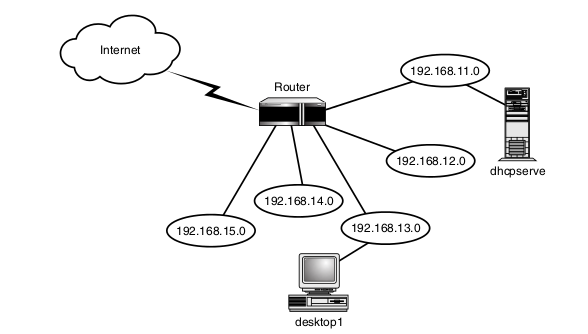
\includegraphics[scale=0.50]{images/2-4.png}
%    \caption{Diagrama - \textit{desktop1} conectada la red 192.168.13.0}
    \label{MAY-4}

    \end{center}
    \end{figure}

    \framebreak
    
    ¿Cómo deduce \textit{dhcpserve} la red de donde proviene el mensaje de
    \textit{desktop1}? Dos maneras posibles:

    \begin{itemize}
        \item Si \textit{desktop1} está en la misma red, el campo 'gateway
        address' debe tener un valor de 0.0.0.0
        \item Si \textit{desktop1} y \textit{dhcpserve} están en segmentos de
        red distintos, entonces un 'relay agent' debe reenviar ese primer
        mensaje y en el proceso añade la dirección de la interfaz por donde
        lo recibió, al campo 'gateway address' de dicho mensaje
    \end{itemize}

    Así \textit{dhcpserve} logra determinar que el mensaje viene de la red
    192.168.13.0, por lo tanto 192.168.12.25 no es una dirección válida.
    Entonces \textit{dhcpserve} envía una respuesta a \textit{desktop1},
    negándole el uso de dicha dirección. Al \textit{desktop1} recibir el
    mensaje, entonces realiza una petición por nueva IP como en el proceso
    'Cuando un computador se conecta por primera vez a la red'.\\[0.2cm]

\end{frame}

\begin{frame}[fragile]{Cuando un computador es eliminado de la red MAY}

   A medida que más computadores se añaden a la sub red 192.168.13.0,
   \textit{dhcpserve} asigna más direcciones a estos nuevos computadores.
   Recordemos que 192.168.13.0 es una dirección de red clase C que solo tiene
   254 direcciones disponibles, eventualmente \textit{dhcpserve} no tendrá
   direcciones para asignar.\\[0.2cm]

   Para evitar eso, \textit{dhcpserve} establece un tiempo de \textit{lease}
   para las direcciones que asigna. Después de que dicho \textit{lease} ha
   expirado, \textit{dhcpserve} 'reclama' dichas direcciones para ser
   reutilizadas por otros clientes DHCP.\\[0.2cm]

   Recordemos que DHCP es un protocolo \textit{Stateless} y por lo tanto no
   diferenciará entre una máquina que se apagó y una máquina que fue removida
   de la red permanentemente.\\[0.2cm]

\end{frame}

\section{Configurando el servidor DHCP} % (fold)
\label{sec:Configurando el servidor DHCP}

% section Configurando el servidor DHCP (end)

\subsection{Especificando la arquitectura de la red} % (fold)
\label{sub:Especificando la arquitectura de la red}

% subsection Especificando la arquitectura de la red (end)

\begin{frame}[allowframebreaks,fragile]{Declaraciones de sub-redes} 
    
    El arquitecto de la red debe describir la arquitectura de la red, al
    servidor DHCP identificando cada una de los IP de las sub-redes, las
    direcciones y las máscaras de red para cada una de las sub-redes.\\[0.2cm]

    Usando dicha información, el servidor DHCP asocia la información que
    recibe, selecciona las IPs apropiadas para asignar a un cliente o
    determina, si un cliente DHCP se ha movido a una nueva
    sub-red.\\[0.2cm]

    \begin{verbatim}
    subnet dirección-de-subred netmask máscara-de-red {
        declaraciones de la subred
    }
    \end{verbatim}

    En esta declaración arriba, 'dirección-de-subred' equivale al IP de la
    sub-red y 'máscara-de-red' a la máscara de sub-red que es necesario usar en
    dicha sub-red. Ambos deben estar escritos en notación decimal.\\[0.2cm]

    Recordemos la figura de las sub-redes de la red MAY:

    \begin{figure}
    \begin{center}

    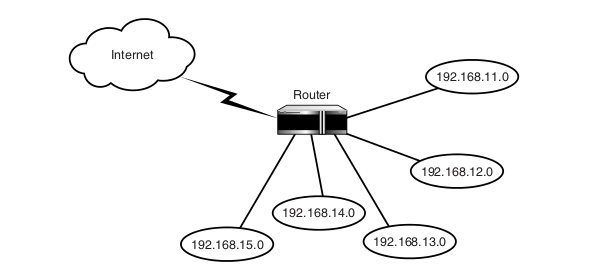
\includegraphics[scale=0.65]{images/2-2.png}
    \caption{Diagrama de sub-redes de la red  MAY} 
    \label{MAY-4}

    \end{center}
    \end{figure}

    Dicha arquitectura de red, se representaría de la siguiente manera:
    \begin{verbatim}
    # subnet de servidores
        subnet 192.168.11.0 netmask 255.255.255.0 {
    }
    # subnet 1 para escritorios
        subnet 192.168.12.0 netmask 255.255.255.0 {
    }
    # subnet 2 para escritorios
        subnet 192.168.13.0 netmask 255.255.255.0 {
    }
    # subnet 3 para escritorios
        subnet 192.168.14.0 netmask 255.255.255.0 {
    }
    # subnet 4 para escritorios
        subnet 192.168.15.0 netmask 255.255.255.0 {
    }
    \end{verbatim}
   
    \framebreak
    
    \textbf{Ejercicio:}\\[0.2cm]

    Procedamos a realizar en la máquina virtual 'server' la configuración de la
    sub-red respectiva para nuestro par de máquinas asignadas.

\end{frame}

\begin{frame}[allowframebreaks,fragile]{Declaración de rangos de asignación a una
sub-red}
    
    Adicional a la definición de sub-redes, el arquitecto de la red debe
    definir los rangos de direcciones dentro de cada sub-red o 'scopes', que
    están disponibles para asignación en dicho servidor DHCP.\\[0.2cm]

    Es importante resaltar que las direcciones asignadas de manera fija por
    cualquier otro mecanismo (manual por ejemplo) deben ser excluidas de los
    rangos definidos como usables para asignación automática o
    dinámica.\\[0.2cm]

    El bloque \textit{range}, se define de la siguiente manera:

    \begin{verbatim}
    range primera-dirección-disponible última-dirección-disponible;
    \end{verbatim}

    Para el ejemplo de la red MAY, tendríamos un bloque como este:

    \begin{verbatim}
    # Server subnet
    subnet 192.168.11.0 netmask 255.255.255.0 {
        range 192.168.11.1 192.168.11.251;
        # 192.168.11.252 reservada para el DHCP 
        # 192.168.11.253 reservada para el DNS 
        # 192.168.11.254 reservada para el router 
    }
    # Staff subnet 1
    subnet 192.168.12.0 netmask 255.255.255.0 {
        range 192.168.12.1 192.168.12.253;
        # 192.168.12.254 reservada para el router 
    }
    # Staff subnet 2
    subnet 192.168.13.0 netmask 255.255.255.0 {
        range 192.168.13.1 192.168.13.253;
        # 192.168.13.254 reservada para el router 
    }
    # Staff subnet 3
    subnet 192.168.14.0 netmask 255.255.255.0 {
        range 192.168.14.1 192.168.14.253;
        # 192.168.14.254 reservada para el router 
    }
    # Staff subnet 4
    subnet 192.168.15.0 netmask 255.255.255.0 {
        range 192.168.15.1 192.168.15.253;
        # 192.168.15.254 reservada para el router 
    }
    \end{verbatim}

    \framebreak

    \textbf{Ejercicio:}\\[0.2cm]

    Procedamos a escribir el respectivo bloque de configuración para el caso
    disponible en nuestro laboratorio.

\end{frame}

\subsection{Parámetros de configuración requeridos} % (fold)

% subsection Parámetros de configuración requeridos (end)

\begin{frame}[allowframebreaks,fragile]{Opciones de configuración}

    DHCP es capaz de proveer otros valores de configuración aparte de la
    dirección IP. De hecho varios parámetros adicionales son necesarios, para
    que un dispositivo pueda comunicarse por TCP/IP con otros dispositivos.
    Dichos parámetros mínimos son:\\[0.2cm]

    \begin{itemize}
        \item La máscara de sub-red
        \item La dirección de al menos un router en la sub-red
        \item La dirección de un servidor DNS
    \end{itemize}

    Estos parámetros se configuran a través de la palabra clave 'option' y
    algunas de las opciones más usadas las estaremos viendo más adelante, su
    sintaxis general es la siguiente:\\[0.2cm]

    \begin{verbatim}
    option nombre-de-la-opción valor-de-la-opción;
    \end{verbatim}

    Si la declaración 'option' aparece dentro de una declaración de sub-red,
    dichos valores serán aplicados a cualquier cliente en la sub-red. En el 
    siguiente ejemplo se usaría una declaración de 'option' para enviar a todos
    los clientes DHCP de la red 192.168.11.0, el router por omisión
    192.168.11.254 
     
    \begin{verbatim}
    # Server subnet
    subnet 192.168.11.0 netmask 255.255.255.0 {
        range 192.168.11.1 192.168.11.251;
        # 192.168.11.252 reservada para el DHCP 
        # 192.168.11.253 reservada para el DNS 
        # 192.168.11.254 reservada para el router 
        option routers 192.168.11.254;
    }
    \end{verbatim}

    \framebreak

    \textbf{Ejercicio:}
    Configure el router por omisión en el bloque de configuración respectivo
    para el ambiente de pruebas disponible, asegúrese de que el 'default
    router' ha sido asignado adecuadamente en el cliente, forzando una
    reconfiguración haciendo 'release' y reinvocándolo con:

    \begin{verbatim}
        dhclient -r && dhclient eth0
    \end{verbatim}

    Y luego revisar la tabla de rutas en cliente con el comando:

    \begin{verbatim}
        netstat -nr
    \end{verbatim}
    
   \framebreak 

    Además de la opción 'routers' el cliente DHCP también necesita una máscara
    de sub-red y un servidor de dominio. Digamos que la red MAY tiene un
    servidor DNS en la dirección 192.168.11.253 y que la máscara de red para
    todas las redes es 255.255.255.0. El bloque de configuración para expresar
    esto sería algo como:\\[0.2cm]
    \begin{verbatim}
# subnet para servidores
    subnet 192.168.11.0 netmask 255.255.255.0 {
        range 192.168.11.1 192.168.11.251;
# 192.168.11.252 reservada para el DHCP 
# 192.168.11.253 reservada para el DNS 
# 192.168.11.254 reservada para el router 
        option routers 192.168.11.254;
        option subnet-mask 255.255.255.0;
        option domain-name-servers 192.168.11.253;
    }
# subnet 1 para escritorios
subnet 192.168.12.0 netmask 255.255.255.0 {
    range 192.168.12.1 192.168.12.253;
# 192.168.12.254 reservada para el router 
    option routers 192.168.12.254;
    option subnet-mask 255.255.255.0;
    option domain-name-servers 192.168.11.253;
}
# subnet 2 para escritorios
subnet 192.168.13.0 netmask 255.255.255.0 {
    range 192.168.13.1 192.168.13.253;
# 192.168.13.254 reservada para el router 
    option routers 192.168.13.254;
    option subnet-mask 255.255.255.0;
    option domain-name-servers 192.168.11.253;
}
# subnet 3 para escritorios
subnet 192.168.14.0 netmask 255.255.255.0 {
    range 192.168.14.1 192.168.14.253;
# 192.168.14.254 reservada para el router 
    option routers 192.168.14.254;
    option subnet-mask 255.255.255.0;
    option domain-name-servers 192.168.11.253;
}
# subnet 4 para escritorios
subnet 192.168.15.0 netmask 255.255.255.0 {
    range 192.168.15.1 192.168.15.253;
# 192.168.15.254 reservada para el router 
    option routers 192.168.15.254;
    option subnet-mask 255.255.255.0;
    option domain-name-servers 192.168.11.253;
}
\end{verbatim}

\framebreak

    \textbf{Ejercicio:} Configure las respectivas líneas de configuración, para
    que el servidor DHCP disponible en el laboratorio envíe la información de
    servidor DNS y máscara de red adecuada para su cliente DHCP. Emplee el
    servidor DNS de su elección. La máscara de red ha de ser
    255.255.255.0\\[0.2cm]

\end{frame}

\subsection{Especificando leases} % (fold)
\label{sub:Especificando leases}

% subsection Especificando leases (end)

\begin{frame}[allowframebreaks,fragile]{Duración de los leases}

    \textit{Lease} se considera al mecanismo a través del que un servidor DHCP sabe
    cuando un dispositivo dejará de usar una dirección IP. La especificación
    del RFC del DHCP establece que el tiempo máximo de un \textit{lease} es
    ${2^{32}}-2$ segundos, equivalente a 49.710 días o alrededor de 135
    años.\\[0.2cm]

    La especificación de DHCP no incluye reglas para la duración de
    \textit{leases}, las políticas deben ser definidas por el arquitecto de la
    red e implementadas por el servidor DHCP. Un cliente DHCP podría solicitar
    un \textit{lease} con una duración particular, pero el servidor DHCP
    siempre eligirá una duración basada en las políticas de \textit{lease}
    definidas por el arquitecto, plasmadas en los archivos de configuración.\\[0.2cm]

\end{frame}

\begin{frame}[allowframebreaks,fragile]{Por omisión, mínimo y máxima duración
de lease}
   
    El servidor DHCP del ISC permite que el arquitecto de la red especifique
    una duración 'por omisión' (default), un tiempo mínimo de duración del \textit{lease} y
    un tiempo máximo de duración del \textit{lease}. El \textit{lease} 'por
    omisión' se usa cuando el cliente no especifica un \textit{lease} en
    particular.\\[0.2cm]
    
    El tiempo mínimo de \textit{lease} se usa para forzar al
    cliente a usar un \textit{lease} superior al que ha solicitado. El máximo
    tiempo de \textit{lease} define el tiempo más prolongado de \textit{lease}
    que puede asignar el servidor. Si un cliente solicita un \textit{lease}
    superior al máximo establecido en la configuración, entonces se le asigna
    el máximo \textit{lease} posible a dicho cliente.\\[0.2cm]

    A continuación un ejemplo de las tres opciones respectivamente:

    \begin{verbatim}
        default-lease-time tiempo-en-segundos:
        min-lease-time tiempo-en-segundos;
        max-lease-time tiempo-en-segundos;
    \end{verbatim}

\end{frame}

\begin{frame}[allowframebreaks,fragile]{Leases en la red MAY}

    Para ver un ejemplo, digamos que en la red MAY la sub-red 192.168.11.0 se usa para servidores,
    que tienen un 'default' de 90 días. Las sub-redes 192.168.12.0, 192.168.13.0,
    y 192.168.14.0 se usan para máquinas de escritorio del personal, que tienen
    asignado un \textit{lease} de 30 días. La sub-red restante, 192.168.15.0, es
    usada para computadores de visitantes y dicho \textit{lease} solo dura 12 horas.\\[0.2cm]

    El bloque de configuración sería algo como:
\begin{verbatim}
option domain-name-servers “dns1.miservidorDNS.com”,
“dns2.miservidorDNS.com”;
option domain-name “dominiogenerico.com”;
# default lease = 30 días, max lease = 45 días
default-lease-time 2592000;
max-lease-time 3888000;
# subnet para servidores
    subnet 192.168.11.0 netmask 255.255.255.0 {
        range 192.168.11.1 192.168.11.251;
# 192.168.11.252 reservada para el DHCP 
# 192.168.11.253 reservada para el DNS 
# 192.168.11.254 reservada para el router 
        option routers 192.168.11.254;
        option subnet-mask 255.255.255.0;
        option domain-name-servers 192.168.11.253;
# lease por default = 90 días, lease máximo = 120 días
        default-lease-time 7776000;
        max-lease-time 10368000;
    }
# subnet 1 para escritorios
subnet 192.168.12.0 netmask 255.255.255.0 {
    range 192.168.12.1 192.168.12.253;
# 192.168.12.254 reservada para el router 
    option routers 192.168.12.254;
    option subnet-mask 255.255.255.0;
    option domain-name-servers 192.168.11.253;
# lease por default = 30 días, lease máximo = 45 días
    default-lease-time 2592000;
    max-lease-time 3888000;
}
# subnet 2 para escritorios
subnet 192.168.13.0 netmask 255.255.255.0 {
    range 192.168.13.1 192.168.13.253;
# 192.168.13.254 reservada para el router 
    option routers 192.168.13.254;
    option subnet-mask 255.255.255.0;
    option domain-name-servers 192.168.11.253;
# lease por default = 30 días, lease máximo = 45 días
    default-lease-time 2592000;
    max-lease-time 3888000;
}
# subnet 3 para escritorios
subnet 192.168.14.0 netmask 255.255.255.0 {
    range 192.168.14.1 192.168.14.253;
# 192.168.14.254 reservada para el router 
    option routers 192.168.14.254;
    option subnet-mask 255.255.255.0;
    option domain-name-servers 192.168.11.253;
# lease por default = 30 días, lease máximo = 45 días
    default-lease-time 2592000;
    max-lease-time 3888000;
}
# subnet 4 para visitantes
subnet 192.168.15.0 netmask 255.255.255.0 {
    range 192.168.15.1 192.168.15.253;
# 192.168.15.254 reservada para el router 
    option routers 192.168.15.254;
    option subnet-mask 255.255.255.0;
    option domain-name-servers 192.168.11.253;
# lease por default = 12 horas, lease máximo = 24 horas
    default-lease-time 43200;
    max-lease-time 86400;
\end{verbatim}

\framebreak

    \textbf{Ejercicio:} Establecer leases 'default', máximos y mínimos para el
    servidor DHCP disponible en el laboratorio con la duración de: 1 semana, 1
    mes y 1 día respectivamente, recuerde que la unidad de tiempo a emplear en
    la configuración, son segundos.\\[0.2cm]
    
\end{frame}

\begin{frame}[allowframebreaks,fragile]{Opciones que son valores globales}

    El ejemplo anterior también nos ayudó a visualizar que se pueden definir
    variables globales, como la duración de los \textit{leases} que
    posteriormente se sobre-escriben con las definiciones locales para cada
    sub-red, permitiéndonos ahorrar líneas de configuración
    innecesaria.\\[0.2cm]
    
\end{frame}

\subsection{Otras opciones de DHCP} % (fold)
\label{sub:Otras opciones de DHCP}

% subsection Otras opciones de DHCP (end)

\begin{frame}[allowframebreaks,fragile]{Configurando otros servicios}
    
    Otras opciones pueden ser usadas como parámetros de configuración que el
    arquitecto de la red podría usar para definir, desde el DHCP server, estas
    se encuentran definidas en el RFC 2132. Algunas muy usadas y otras
    totalmente en desuso, a continuación un listado:

    \begin{verbatim}
swap-server         time-servers            domain-name-servers
log-servers         cookie-servers          lpr-servers
nis-servers         ntp-servers             netbios-name-servers
font-servers        x-display-managers      nis-plus-servers
tftp-server-name    smtp-server             pop-server
nntp-server         www-server              finger-server
irc-server          impress-server          streettalk-server 
    \end{verbatim} 

\end{frame}



\end{document}
